%% LyX 2.0.6 created this file.  For more info, see http://www.lyx.org/.
%% Do not edit unless you really know what you are doing.
\documentclass[12pt,english]{paper}
\usepackage[T1]{fontenc}
\usepackage[latin9]{inputenc}
\usepackage{listings}
\setlength{\parskip}{\smallskipamount}
\setlength{\parindent}{0pt}
\usepackage{url}
\usepackage{graphicx}
\usepackage{setspace}
\doublespacing
\usepackage{babel}
\begin{document}

\title{BPL Lab User Guide}
\maketitle
\begin{abstract}
Web site 'rscript.cisdd.org' offers some basic tools to perform research
on building sensors data: visualization, basic statistics and forecast. 

Developed in Django/Python, the application data model is based on
Panda objects and exposes a small set of Python functionalities to
the user.

\includegraphics[clip,scale=0.3]{general}
\end{abstract}

\section{Data Sources and graphing}

The site is provided with a collection of data coming from John Jay
building sensors. As of today it contains about one year of every
15 minutes observations of a thousand sensors. Data are stored on
a local slqlite database and updated asynchronously by a separate
process. This architecture guarantees a quick and constant access
time to data this allowing complex computations in a reasonable amount
of time.

Data are presented in a tree, ordered by type, location and name:

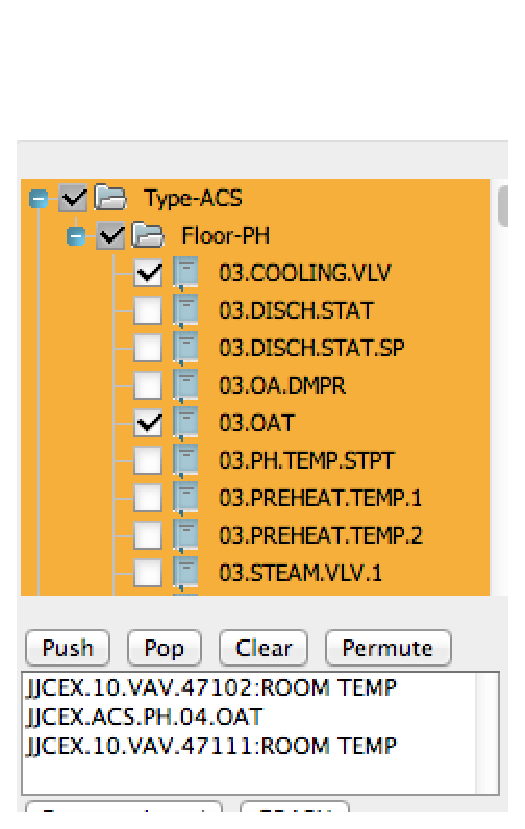
\includegraphics[scale=0.7]{fig1}

From there, user can choose one or several sensor, an entire floor
or an entire category. Once chosen, sensors are selected for analysis
by pressing 'Push' to transfer selection into the selection stack.


\subsection{The selection stack}

Selection stack contains reference data that will be used during the
analysis session. Data are implicitly indexed (0,1,2 etc.) and index
references are used later on during the filtering and the formatting
phases. To modify the order sequence the button 'Permute' will swap
selected sensor with the top of the stack. 'Clear' will empty the
stack and 'Pop' will remove the selected input.


\subsection{The filter box}

Right under the selection stack we have the filter box: it consists
in an array of Python lambda functions in 'x' the user will write
to filter out input data.

The filters are separated by ';' followed by a return. Each line matches
with the corresponding sensor from the sensor stack, starting with
the time axis:

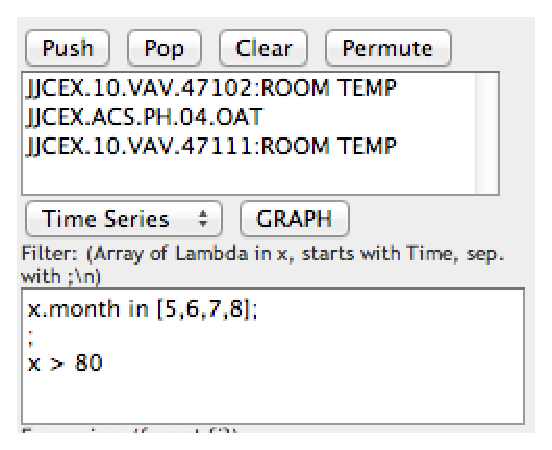
\includegraphics[clip,scale=0.7]{fig2}

In this example the first line is used to filters time axis, then
sensor 1 from the stack, followed by sensor 2 , etc. Here we want
data for which the observation month is either 5,6,7 or 8. Then there
is no constraint on sensor 1, and sensor 2 must have values greater
than 80.


\subsubsection{The time axis filter}

The first line is a Python boolean lambda function in 'x' where 'x'
is the time, and more precisely it is a Python datetime object on
which the following members are defined:

\begin{lstlisting}
x.year, x.month, x.day, x.hour, x.minute, x.second, x.microsecond
\end{lstlisting}


Also some functions:

\begin{lstlisting}
x.weekday(), x.replace()
\end{lstlisting}


And comparison with a datetime object:

\begin{lstlisting}
x >= datetime(2013,2,1)
\end{lstlisting}


The complete documentation is available at :

\url{https://docs.python.org/2/library/datetime.html#datetime-objects}


\subsubsection{lambda x}

Almost all the sensors are represented by float 64 values, thus filters
will apply to Python floats. Boolean expression and math functions
are allowed, so it is possible to build complex queries, but sub function
definitions are not authorized. Math functions must be prefixed by
'math.' . Example :

\begin{lstlisting}
math.log(x) > 2 and math.sin(x) == math.pi;
\end{lstlisting}


More on Python expressions:

\url{https://docs.python.org/2/reference/expressions.html}

More on Python math module:

\url{https://docs.python.org/2/library/math.html}


\subsection{The expression boxes}

Under the filter text field there is another field we use to format
data output. It is in fact like a Python string format expression,
but it is destined to be evaluated by the Python interpreter within
the context of the analysis: Every input is represented by a format
field within brackets: \{0\},\{1\}, etc.

\includegraphics[bb=0bp 0bp 249bp 105bp,clip]{fig3}

There is two expression boxes: one for graphing of data, and the other
for learning.

Behind these templates are Pandas objects, more precisely Pandas columns.
One has to see the output has a table where every column represents
a particular sensor (plus the time). What is evaluated prior to graph
is in fact a formatted expression. Basic arithmetics and special functions
are allowed, as well as basic boolean expressions (for which we will
prefer using the filter box because the syntax is much lighter).
\begin{itemize}
\item Reordering the output is then permitted : 
\begin{lstlisting}
{1},{0},{2}
\end{lstlisting}
 will display sensor 2, sensor 1 then sensor 3. This will be useful
during the forecast/training phase. Note : counting must starts at
0 and increments by 1.
\item Basic arithmetic:
\begin{lstlisting}
{1} - {0}, abs({1} - {0}), {1} - {0}/{1}*200
\end{lstlisting}

\item Basic Pandas built-ins (only those that returns a set) :
\begin{lstlisting}
{0}.diff(), {0}.pct_change(),{0}.cumsum()
\end{lstlisting}

\item Special 'apply' function that allows math or lambda expressions:
\begin{lstlisting}
{0}.apply(math.sin), {0}.apply(lambda x : x if x <= 0 else math.log(x))
\end{lstlisting}

\item Special field '\{t\}' to access time axis: \{t\} represents a datetime
object
\begin{lstlisting}
{t}.apply(lambda x : x.hour % 4)
{t}.apply(lambda x : x.weekday())
\end{lstlisting}

\end{itemize}
The complete Pandas documentation on basic functions and expressions
is available here:

\url{http://pandas.pydata.org/pandas-docs/stable/basics.html#function-application}


\subsection{Graph Types}

Several graph types can be created. The following menu gives the possible
choices:

\includegraphics[clip,scale=0.7]{graph}

Data will be filtered out according to the filter box and several
graphs will be created following the template defined in the format
box.
\begin{itemize}
\item Time Series: Y's are the data, X is the time.
\item Moving Std: That will compute, for every data, the MA plus +/- 2 standard
deviations computed on a rolling period of 20 ticks (20 {*} 15 minutes).
It shows trend and values which are outside the STD envelope are likely
to be 'abnormal'.
\item XY : X axis is the first entry corresponding to the forma, Y's are
the next ones. By default X is going to be the element on top of the
stack. But it is possible to graph more complex expressions; for instance
\{2\}-\{1\},\{0\} in the format box will display (sensor 2 - sensor
1) in X and (sensor 0) in Y. XY values are sorted and unique.
\item Correl: Shows a rolling windows (20 elements) of cross correlations
between the first set of values compared to the others. 
\item Frequencies: Show an histogram of the value distribution, only for
the first element (for readability reasons)
\end{itemize}
All this types are compatible with filters and formats detailed above.


\section{Persistence}

The lab allows some basic persistence, it is possible to save/load
a context under a given name. The context consists in :
\begin{itemize}
\item sensor list
\item graph type
\item filter box and expression boxes
\item MAW and training size 
\item Machine type and learned set (if it exists)
\end{itemize}
To create a new context, simply type a name in the field :

\includegraphics[clip,scale=0.7]{p}

The new name is then added to the menu and can be loaded.

Training a new set will automatically save it, and if a name is not
provided then it will be saved under generic name 'tmp'. 

Context are stored on the server so every user can see them and thus
share their own sets.

Deleting a set is not possible for now and must be manually done by
the developers.


\section{Machine Learning}

BPL Research offers some machine learning features: from a given set
of data a machine can be trained and forecasts a specific output.

Machine input and output are defined the same way as graphs: Filters
are applied to the selected stack and an expression is eventually
computed. 

From there, 'Learn' button will start training. The reference output
is the first value defined in the Expression Box (by default it is
the top sensor on the stack) at T + 1 tick.

Inputs are the other values at T. Learning results are shown as a
graph comparing training values to forecast.

Training parameters are :
\begin{itemize}
\item MAW : moving average period (in ticks). A training/forecast can be
performed on moving average data instead of raw data. A MAW of 1 means
no moving average.
\item Train size: size of training set as a percentage of the input set.
The training set is uniformely sampled from the data set.
\item Machine type: as of today : K-Nearest neighbor, Perceptron, Forest
tree and SVM. 
\end{itemize}
Machine learning is entirely based on the Python Sci Kit libraries,
and adding new models can be done easily. More information on SciKit
:

\url{http://scikit-learn.org/stable/index.html}

So far, we have noticed that the best regressor seems to be SVM.

After training ('Learn' button), the trained set is saved as part
of the selected configuration and it's then possible to run it against
a different set of parameters, by modifying the sensor stack or the
expression box. Beware of the fact that the number of input must be
the same. 


\section{Notes on code}

The entire application is based on Python, the front end being HTML
and JavaScript, and the framework is based on Django. 

Source is available from CVS : :pserver:eric@rscript.cisdd.org:/home/eric/cvsrepo
\end{document}
